\section{Architektura systemu WIP}
\label{sec:Architektura_systemu}

\subsection{Przegląd architektury}

System został zaprojektowany jako zautomatyzowany pipeline CI/CD dla modeli uczenia maszynowego. Obejmuje cały cykl życia modelu: od dodania danych treningowych, przez walidację danych i trening, aż po wybór najlepszego modelu i wdrożenie.

Architektura opiera się na trzech głównych obszarach:
\begin{itemize}
  \item kontrola wersji kodu i danych,
  \item uruchamianie zadań i wdrożeń w kontenerach,
  \item rejestrowanie eksperymentów oraz wersji modeli.
\end{itemize}

Punktem centralnym jest repozytorium Git. To w nim przechowywany jest kod, konfiguracja oraz metadane danych. Każdy push lub merge może uruchomić automatyczne procesy w GitHub Actions \cite{github_actions_docs}. Dzięki temu użytkownik nie musi ręcznie wykonywać większości kroków operacyjnych.

Część obliczeniowa działa w chmurze AWS. Zasoby są uruchamiane tylko wtedy, gdy są potrzebne, na przykład na czas treningu lub pobrania modelu. Po zakończeniu pracy instancja jest zatrzymywana, aby ograniczyć koszty. Szczegółowe uzasadnienie takich decyzji znajduje się we wprowadzeniu w sekcji \ref{sec:Wprowadzenie}.

W projekcie wykorzystano model U-Net do segmentacji semantycznej obrazów wodomierzy. Metryki Dice oraz IoU są używane w bramce jakości, która decyduje, czy nowa wersja modelu może zostać uznana za lepszą od obecnej.

\subsection{Komponenty systemu}

\subsubsection{Warstwa kontroli wersji}

Git odpowiada za wersjonowanie kodu, konfiguracji oraz metadanych związanych z danymi treningowymi. Repozytorium można podzielić na trzy logiczne części.

\paragraph{Kod modelu i skrypty treningowe}\mbox{}\\
Ta część zawiera implementację modelu U-Net w PyTorch oraz skrypty odpowiedzialne za przygotowanie danych, trening i walidację. Ponieważ kod jest wersjonowany, można odtworzyć, w jakich warunkach trenowano konkretną wersję modelu.

\paragraph{Dane treningowe}\mbox{}\\
Domyślną metodą zarządzania danymi treningowymi w systemie jest DVC \cite{dvc_docs}. Repozytorium Git przechowuje wtedy jedynie metadane i pliki śledzące (na przykład \texttt{.dvc} oraz \texttt{dvc.lock}), natomiast właściwe obrazy i maski znajdują się w Amazon S3. Takie podejście skaluje się znacznie lepiej niż trzymanie dużych plików w Git i pozwala na wersjonowanie danych w sposób spójny z wersjonowaniem kodu.

W wariancie proof of concept dopuszczono również możliwość przechowywania małych zbiorów danych bezpośrednio w repozytorium, aby uprościć szybkie testy. Należy jednak zaznaczyć, że użycie DVC wiąże się z dodatkowym krokiem \texttt{dvc pull}, który w praktyce może zauważalnie wydłużyć czas działania pipeline, szczególnie przy większych zbiorach danych.

\paragraph{Infrastruktura jako kod}\mbox{}\\
Definicja infrastruktury jest utrzymywana w kodzie, głównie jako moduły Terraform \cite{hashicorp_terraform} oraz konfiguracje Helm \cite{helm_docs}. Dzięki temu środowisko można odtworzyć w sposób powtarzalny, a zmiany infrastruktury są widoczne w historii repozytorium.

\subsubsection{Warstwa uruchamiania procesów}

\paragraph{GitHub Actions}\mbox{}\\
GitHub Actions pełni rolę głównego mechanizmu uruchamiania procesów CI/CD. W projekcie wykorzystano kilka workflow, z których najważniejsze realizują następujące zadania:
\begin{itemize}
  \item walidacja danych treningowych,
  \item uruchomienie treningu modelu i zebranie wyników,
  \item uruchamianie i zatrzymywanie instancji EC2,
  \item testy jakości kodu i testy jednostkowe,
  \item obsługa procesu dodania danych i utworzenia pull requesta.
\end{itemize}

\paragraph{Instancja EC2 i k3s}\mbox{}\\
Zamiast zarządzanego klastra Kubernetes zastosowano k3s \cite{k3s_docs} uruchomiony na pojedynczej instancji EC2. To podejście jest wystarczające dla projektu proof of concept i pozwala znacząco ograniczyć koszty. Na instancji działa klaster k3s oraz usługi potrzebne do treningu i wdrożeń.

\paragraph{MLflow}\mbox{}\\
MLflow \cite{zaharia2018mlflow} odpowiada za dwie rzeczy. Po pierwsze zapisuje przebieg eksperymentów, czyli metryki, parametry oraz artefakty treningu. Po drugie przechowuje wersje modeli i ich status, na przykład Production lub Archived. W tym projekcie metadane są przechowywane w bazie lokalnej na instancji EC2, a artefakty trafiają do S3.

\subsubsection{Warstwa przechowywania danych}

\paragraph{Amazon S3}\mbox{}\\
S3 jest używane jako trwałe miejsce przechowywania. W systemie trafiają tam głównie artefakty z MLflow, takie jak wagi modeli i logi. Opcjonalnie S3 może też być wykorzystywane do przechowywania danych treningowych, jeśli używany jest DVC.

\paragraph{Amazon ECR}\mbox{}\\
ECR służy jako rejestr obrazów Docker. Po zaakceptowaniu modelu przez bramkę jakości obraz kontenera jest budowany i wysyłany do ECR, a następnie wdrażany na klaster k3s.

Warto zaznaczyć, że jeśli dane są przechowywane w DVC, etap przygotowania środowiska obejmuje dodatkowe pobranie danych z S3, co jest jednym z głównych źródeł wydłużenia czasu całego workflow treningowego.

\subsubsection{Warstwa monitorowania}

System zawiera komponenty monitoringu oparte na Prometheus \cite{prometheus_docs} oraz Grafana. Prometheus zbiera metryki z endpointu \texttt{/metrics} udostępnionego przez API modelu, a Grafana prezentuje je w postaci dashboardów. Szczegóły konfiguracji stosu monitorowania opisane są w rozdziale \ref{sec:Implementacja_wdrozenia}.

\subsection{Diagram architektury}

\begin{figure}[H]
\centering
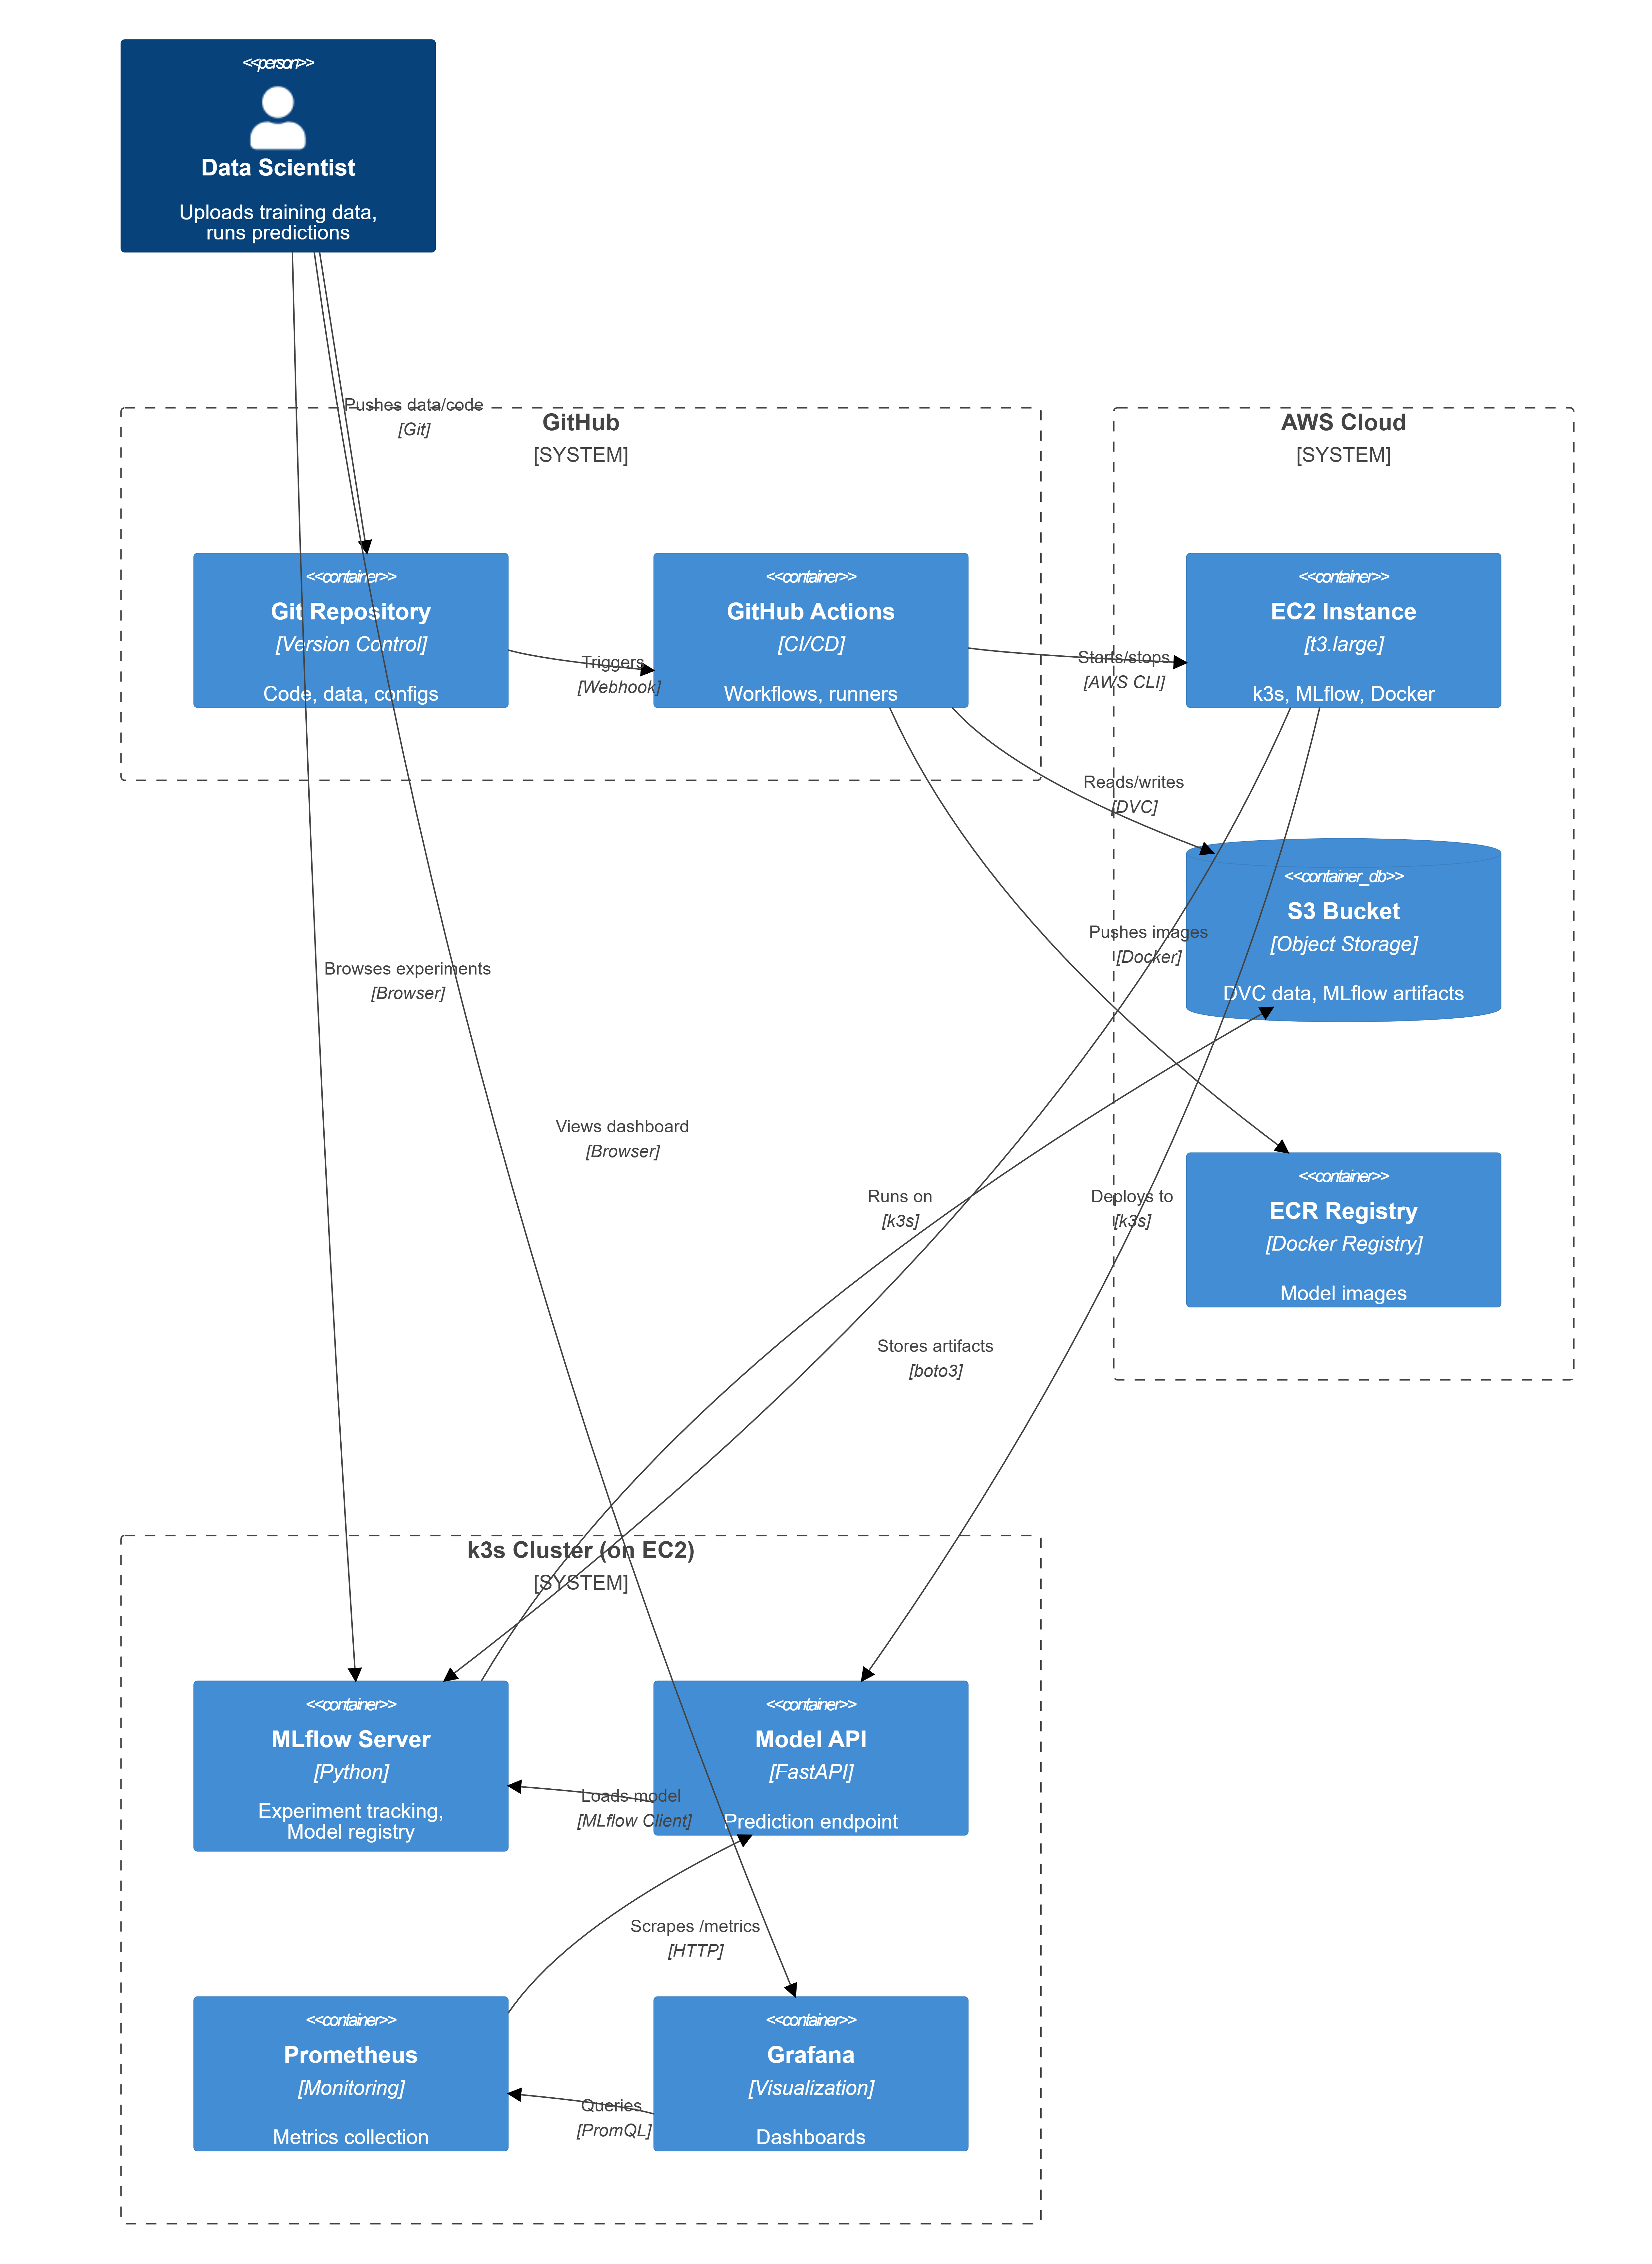
\includegraphics[width=\textwidth]{img/02_architektura_systemu/architecture-overview.png}
\caption{Diagram kontekstowy C4 przedstawiający główne komponenty systemu oraz ich interakcje}
\label{fig:architecture-overview}
\end{figure}

Rysunek \ref{fig:architecture-overview} przedstawia kontekst systemu w notacji C4. Użytkownik pracuje z repozytorium Git, a automatyzacja realizowana jest przez GitHub Actions. Workflow zarządzają zasobami AWS, uruchamiają instancję EC2 i wykonują zadania treningowe oraz wdrożeniowe. Na EC2 działa klaster k3s, w którym uruchomione są MLflow, API modelu oraz narzędzia monitoringu. Artefakty modelu są przechowywane w S3, a obrazy kontenerów w ECR.

\subsection{Przepływ danych w systemie}

\begin{figure}[H]
\centering
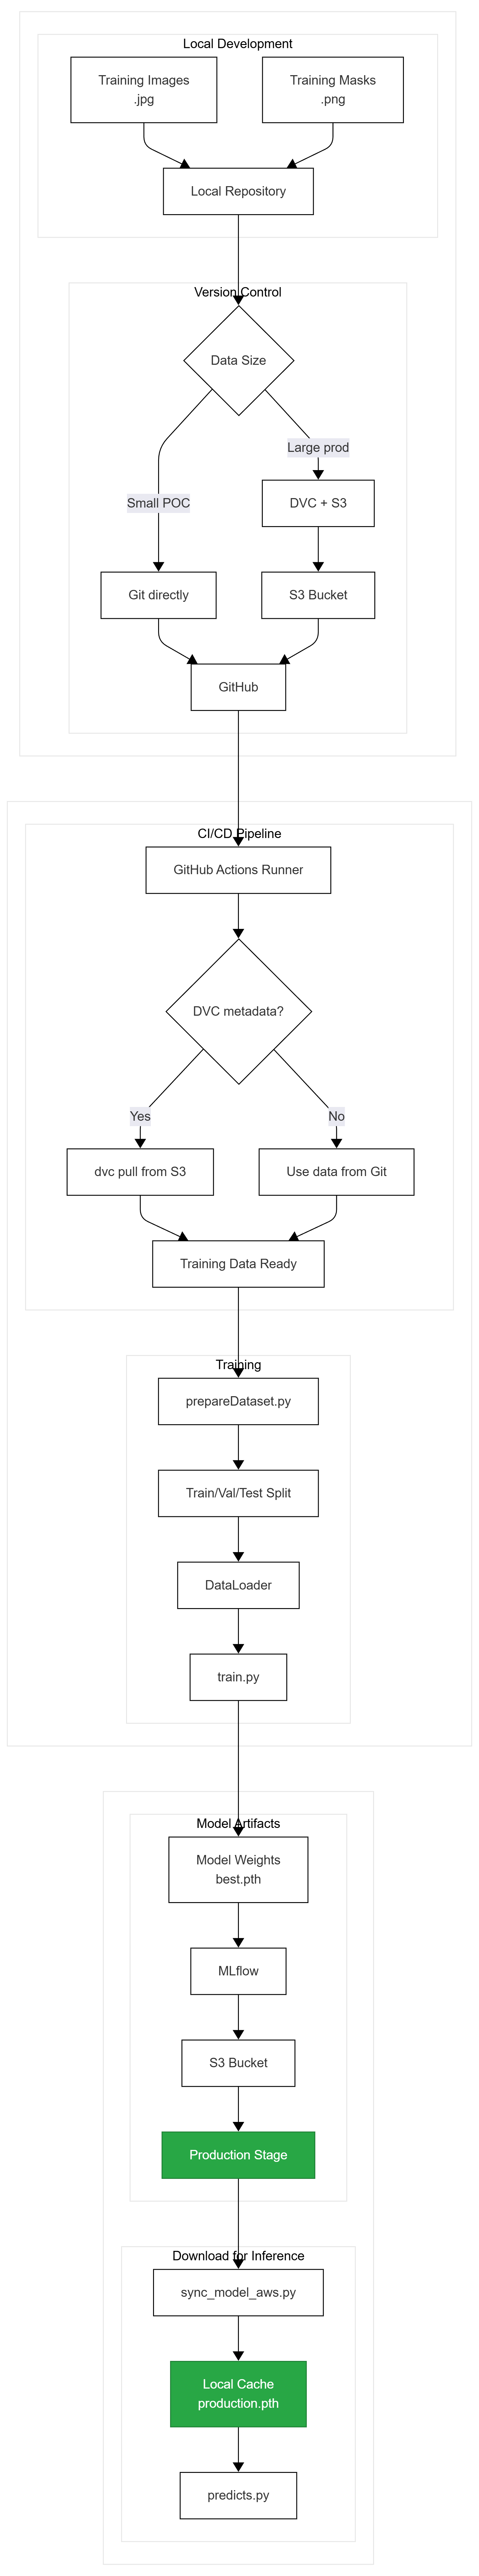
\includegraphics[scale=0.09]{img/02_architektura_systemu/data-flow.png}
\caption{Diagram przepływu danych treningowych przez system}
\label{fig:data-flow}
\end{figure}

Rysunek \ref{fig:data-flow} pokazuje drogę danych od lokalnego repozytorium do artefaktów produkcyjnych. Dane są wersjonowane przez DVC, a następnie pobierane przez runner GitHub Actions. Skrypty przygotowują podział danych, trening generuje wagi modelu, a wynik jest rejestrowany w MLflow. Model Production może zostać pobrany lokalnie i użyty do predykcji.
